\subsection{AwesomeFigures visualization of computational cost and five selection criteria}
\label{sec:awesomefigures-mle}
Figures~\ref{fig:gcv-six-orders}--\ref{fig:five-criteria-times} are
generated from archived machine-recorded CSV files through the
\texttt{awesomefigures} Python library, with vector PDF export at the
measured text width and typography of the official Springer Nature
manuscript. Browser-compatible SVG variants accompany the documentation.
No benchmark values are generated during plotting.

\begin{figure}[tbp]
\centering
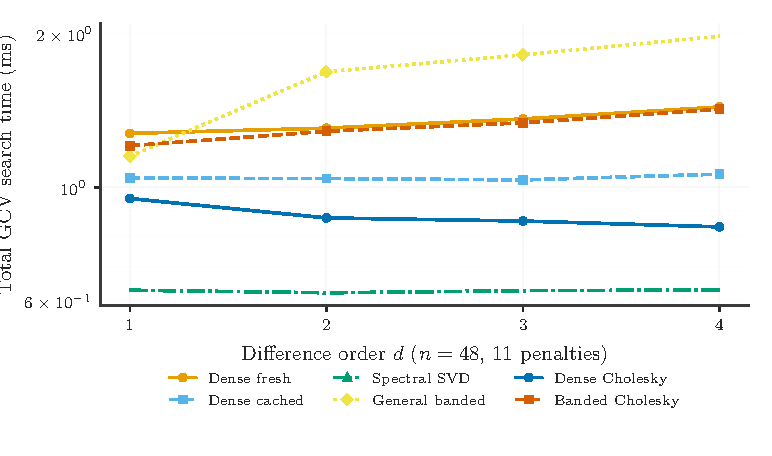
\includegraphics{figures/gcv_solver_by_order.pdf}
\caption{Measured end-to-end classical GCV grid selection for six numerical
solvers and finite-difference order $d=1,\ldots,4$, $n=48$, $M=11$
positive finite log-penalty candidates, fixed $\mu=0$, one series,
and warm setup, on the recorded GitHub-hosted Linux machine.
Each method computes its own EDF; general banded and banded Cholesky
are distinct factorizations. The vertical axis is logarithmic.}
\label{fig:gcv-six-orders}
\end{figure}

\begin{figure}[tbp]
\centering
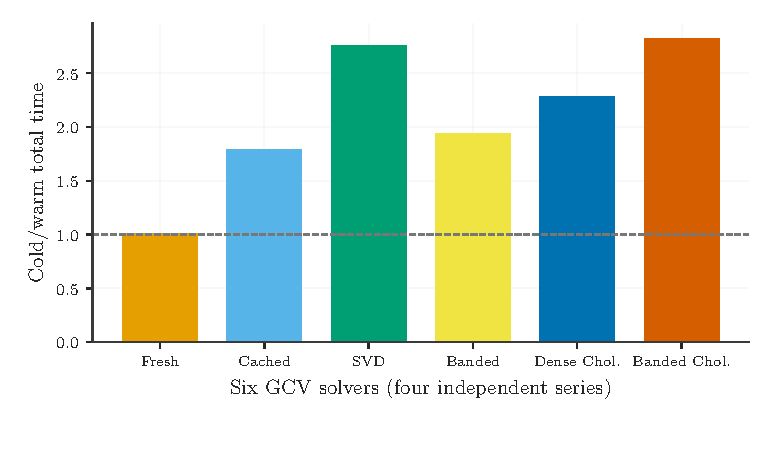
\includegraphics{figures/gcv_repeated_search.pdf}
\caption{Ratio of measured cold to warm complete GCV selection time
for four independent series revisiting identical finite penalties
($n=48$, $d=2$, $M=11$, fixed $\mu=0$).
Ratios above one favor shared preprocessing; a Cholesky factor may
be reused for a repeated penalty but not for a different one.}
\label{fig:gcv-repeated}
\end{figure}

The comparison of statistical selection criteria also includes
Gaussian profiled marginal maximum likelihood (MLE) already available
as \texttt{criterion="mle"}, alongside fixed-mean CV, GCV, AICc
and BIC. This MLE profiles the observation variance, integrates
the penalized latent coordinates and excludes the unpenalized polynomial
null space. It conditions on a fixed numerical difference-reference mean
$\mu$, not on an estimated joint $(\mu,\lambda)$ likelihood.
MLE is a \emph{criterion}, not a seventh matrix factorization.
At $\lambda=0$ the Gaussian latent model is improper and MLE assigns an
infinite score. Raw scores across the five criteria are not comparable.

The search-coordinate experiment uses the same 16 candidate
smoothness targets ($0,0.1,\ldots,1$ plus
$0.95,0.99,0.999,0.9999,0.999999$).
Mapped penalty first computes $S^{-1}(s_j)$ and reuses the resulting
penalties for all five criteria. Native $S$ supplies those same targets
to each public selector, repeating the inversions; both score
identical candidates up to numerical tolerance.
An independent log-penalty grid has 16 values including both endpoints
but different interior candidates, so finite-grid minima need not coincide.
The mapped and native-S selection times exclude shared SVD setup, and
the one-time shared mapping cost is recorded separately. The scope
differs from the six-backend GCV experiment above.

\begin{figure}[tbp]
\centering
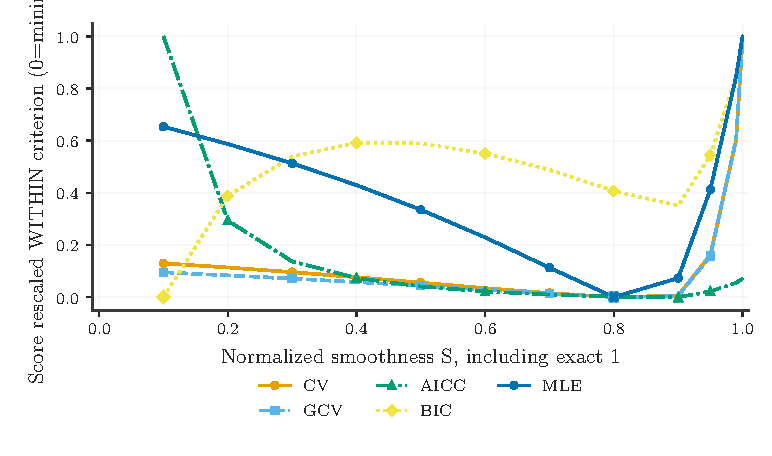
\includegraphics{figures/criteria_with_mle_s_paths.pdf}
\caption{CV, GCV, AICc, BIC and conditional profiled marginal MLE
score profiles on the same mapped smoothness targets for a seeded
synthetic series ($n=60$, $d=2$, fixed $\mu=0$).
Each profile is shifted and rescaled \emph{within its own criterion}
to display shape and minima; ordinate values cannot be compared across
criteria. The exact $S=1$ limit is evaluated.}
\label{fig:five-criteria-paths}
\end{figure}

\begin{figure}[tbp]
\centering
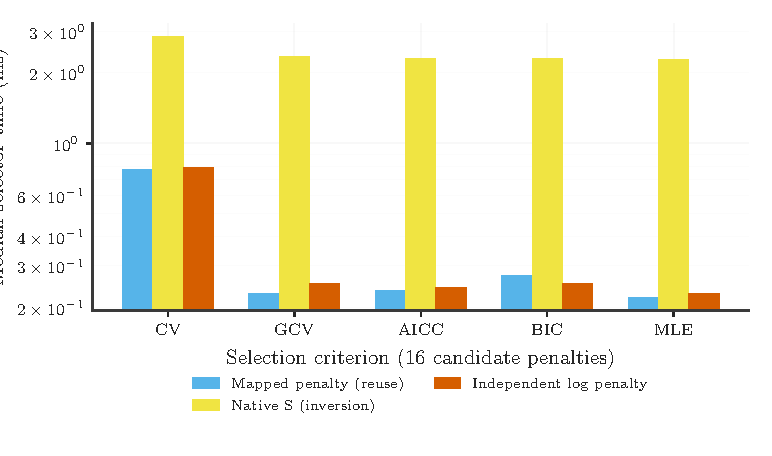
\includegraphics{figures/criteria_with_mle_search_time.pdf}
\caption{Measured public spectral \texttt{select\_lambda} time over
16 candidate points, including MLE and four classical criteria
($n=60$, $d=2$, fixed $\mu=0$). Mapped $\lambda$ and native $S$
use identical penalties but the latter repeats numerical inversion.
The independent log-penalty grid has different interior values.
The logarithmic ordinate excludes common spectral setup and
shared inversion preprocessing (recorded in separate CSV fields).}
\label{fig:five-criteria-times}
\end{figure}

Both studies also evaluate fixed $\mu=0.15$; the selection script
supports additional orders. Single-host repeated timings are
descriptive, not corrected multi-seed inferential evidence or
forecast-horizon validation. Source rows, mappings, and platform
metadata are archived in
\texttt{paper/benchmarks/selection\_coordinate\_reference/}.
